\documentclass[titlepage]{book}

% PACKAGES

\usepackage[fontsize=13pt]{fontsize}
\usepackage{afterpage}
\usepackage{amsmath, amssymb}
\usepackage{slashed}
\usepackage[utf8]{inputenc}
\usepackage{chngcntr}
\usepackage{blindtext}
\usepackage[labelsep=space]{caption}
\usepackage{enumitem}
\usepackage{fancyhdr}
\usepackage[T1]{fontenc}
\usepackage[bottom=6.5em]{geometry}
\usepackage{graphicx}
\usepackage{gensymb}
\usepackage[hyperfootnotes=false,linktoc=page,pdfpagelayout=TwoPageRight]{hyperref}
\usepackage{lettrine}
% \usepackage{cfr-lm}
\usepackage{makecell}
\usepackage{mathtools}
\usepackage{multicol}
\usepackage[defaultlines=4,all]{nowidow}
\usepackage{titlesec}
\usepackage[titles]{tocloft}
\usepackage{wrapfig}
\usepackage{lipsum}
\usepackage{xcolor}
\usepackage{tikz-feynman}
\tikzfeynmanset{compat=1.1.0}
\usepackage{simpler-wick}
% IMPORTS

% MATH SHORTHANDS
% Partial Differential of #1 w.r.t. #2
\newcommand{\dpartial}[2]{\frac{\partial #1}{\partial #2}}

% \ceil{x} instead of \lceil x \rceil
% Same for \floor{x}
\DeclarePairedDelimiter\ceil{\lceil}{\rceil}
\DeclarePairedDelimiter\floor{\lfloor}{\rfloor}
\newcommand{\abs}[1]{\left| #1 \right|}

% Auto-resize () and []
\newcommand*\autoop{\left(}
\newcommand*\autocp{\right)}
\newcommand*\autoob{\left[}
\newcommand*\autocb{\right]}
\AtBeginDocument {%
   \mathcode`( 32768
   \mathcode`) 32768
   \mathcode`[ 32768
   \mathcode`] 32768
   \begingroup
       \lccode`\~`(
       \lowercase{%
   \endgroup
       \let~\autoop
   }\begingroup
       \lccode`\~`)
       \lowercase{%
   \endgroup
       \let~\autocp
   }\begingroup
       \lccode`\~`[
       \lowercase{%
   \endgroup
       \let~\autoob
   }\begingroup
       \lccode`\~`]
       \lowercase{%
   \endgroup
       \let~\autocb
}}
\delimiterfactor 1001
\makeatletter
\AtBeginDocument {%
          \def\resetMathstrut@{%
           \setbox\z@\hbox{\the\textfont\symoperators\char40}%
           \ht\Mathstrutbox@\ht\z@ \dp\Mathstrutbox@\dp\z@}%
}%
\makeatother

\newcommand{\vecbr}[1]{\langle #1 \rangle}

% Unit vectors

\newcommand{\ui}{\hat{\imath}}
\newcommand{\uj}{\hat{\jmath}}
\newcommand{\uk}{\hat{k}}
\newcommand{\V}{\vec{V}}

% Common expressions

\newcommand{\half}[1]{\frac{#1}{2}}
\newcommand{\recip}[1]{\frac{1}{#1}}
\newcommand{\invsqrt}[1]{\recip{\sqrt{#1}}}
\newcommand{\halfpi}{\half{\pi}}

% Integral evaluation bar
\newcommand{\windbar}[2]{\Big|_{#1}^{#2}}
\newcommand{\rightinfwindbar}[0]{\Big|_{0}^\infty}
\newcommand{\leftinfwindbar}[0]{\Big|_{-\infty}^0}

% Column type "L" for tabular environment, contents of column are in display mode by default
\newcolumntype{L}{>{$}l<{$}}

% Circled single character (used for state machine notation)

\newcommand{\state}[1]{\large\protect\textcircled{\textbf{\small#1}}}

% FORMATTING
% Remove section numbers
\makeatletter
\renewcommand{\@seccntformat}[1]{}
\makeatother
% Indent text within section
% \leftskip=2em
% Center section headings
\titleformat{\section}[block]{\Large\bfseries\filcenter}{}{1em}{}
% `enumerate` environment uses (\alph) format
\setlist[enumerate]{label=(\alph*)}

\newcommand{\shrule}{\\ \centerline{\rule{13cm}{0.4pt}}}

% QUANTUM 

\usepackage{mathtools}
\DeclarePairedDelimiter\bra{\langle}{\rvert}
\DeclarePairedDelimiter\ket{\lvert}{\rangle}
\DeclarePairedDelimiterX\braket[2]{\langle}{\rangle}{#1 \delimsize\vert #2}
\DeclarePairedDelimiterX\brakaket[3]{\langle}{\rangle}{#1 \delimsize\vert #2 \delimsize\vert #3}
\newcommand{\tbra}[1]{$\bra{#1}$}
\newcommand{\tket}[1]{$\ket{#1}$}
\newcommand{\tbraket}[2]{$\braket{1}{2}$}
\newcommand{\infint}[0]{\int_{-\infty}^{\infty}}
\newcommand{\rightinfint}[0]{\int_0^\infty}
\newcommand{\leftinfint}[0]{\int_{-\infty}^0}
\newcommand{\wavefuncint}[1]{\infint|#1|^2}
\newcommand{\ham}[0]{\hat{H}}


% PAGE HEADERS

\let\Sectionmark\sectionmark
\def\sectionmark#1{\def\Sectionname{#1}\Sectionmark{#1}}

\let\Subsectionmark\subsectionmark
\def\subsectionmark#1{\def\Subsectionname{#1}\Subsectionmark{#1}}

\pagestyle{fancy}
\fancyhf{}
\fancyhead[LE]{\thepage}
\fancyhead[RE]{\Sectionname}
\fancyhead[LO]{\MakeUppercase{\Subsectionname}}
\fancyhead[RO]{\thepage}
\renewcommand{\headrulewidth}{0pt}

% GRAPHICS

\graphicspath{ {./images/} }

% SECTION FORMAT

\counterwithout{subsection}{section}

\renewcommand{\thesection}{PART \Roman{section}}
\renewcommand{\thesubsection}{\Roman{subsection}}
\renewcommand{\thesubsubsection}{\Roman{subsubsection}}

\newcommand{\subsectionbreak}{\newpage}

\titleformat{\section}[display]{\Large\bfseries\filcenter}{\thesection}{.5em}{}
\titleformat{\subsection}[display]{\large\bfseries\filcenter}{\thesubsection}{0em}{\uppercase}

\counterwithin*{footnote}{page}

% FIGURES

\renewcommand{\thefigure}{\roman{figure}}

\renewcommand{\figurename}{\textsc{Fig.}}

\newcommand{\fig}[3]{
    \begin{figure}[h]
        \centering
        \includegraphics[width=\linewidth]{#1}
        \textbf{\caption{#2}}
        \label{fig:#3}
    \end{figure}
}

% EQUATIONS

\newcommand{\eq}[1]{
    \begin{equation*}
    \begin{split}
        #1
    \end{split}
    \end{equation*}
}

\newcommand{\eqnum}[1]{
    \begin{equation}
    \begin{split}
        #1
    \end{split}
    \end{equation}
}

% OLDSTYLENUMS

\DeclareMathSymbol{0}{\mathalpha}{letters}{`0}
\DeclareMathSymbol{1}{\mathalpha}{letters}{`1}
\DeclareMathSymbol{2}{\mathalpha}{letters}{`2}
\DeclareMathSymbol{3}{\mathalpha}{letters}{`3}
\DeclareMathSymbol{4}{\mathalpha}{letters}{`4}
\DeclareMathSymbol{5}{\mathalpha}{letters}{`5}
\DeclareMathSymbol{6}{\mathalpha}{letters}{`6}
\DeclareMathSymbol{7}{\mathalpha}{letters}{`7}
\DeclareMathSymbol{8}{\mathalpha}{letters}{`8}
\DeclareMathSymbol{9}{\mathalpha}{letters}{`9}

% REFERENCES

\hypersetup{
    colorlinks=false,
    linkbordercolor={0 0 0},
    pdfborderstyle={/S/U/W 0.0}
}

\newcommand{\secref}[1]{\hyperref[sec:#1]{Section #1}}

\newcommand{\figref}[1]{\hyperref[fig:#1]{Fig. #1}}

% LARGE FIRST LETTER OF SECTION

\newcommand{\firstword}[2]{
    \lettrine[lines=3,nindent=0em,findent=0.5em,realheight]{#1}{#2}
}

% TABLE OF CONTENTS FORMAT

\renewcommand{\contentsname}{CONTENTS}
\renewcommand{\cfttoctitlefont}{\hfil\bfseries\fontsize{15pt}{0pt}\selectfont}
\renewcommand{\cftaftertoctitleskip}{0.5\baselineskip}
\renewcommand{\cftsecfont}{\bfseries}

\addtolength{\cftsecnumwidth}{40pt}
\addtolength{\cftsubsecnumwidth}{10pt}
\setlength{\cftbeforetoctitleskip}{-3em}

\setcounter{tocdepth}{4}
\setcounter{secnumdepth}{4}

% TITLE SETUP

\title{\textbf{\huge{A cross section calculation handbook for students}}}

\author{
    Dacheng Xu
}

\date{}

% MISC

\newcommand{\aether}[0]{\ae ther}

\newcommand{\letlist}[1]{
    \begin{enumerate}[label=(\emph{\alph*})]
        #1
    \end{enumerate}
}

% DOCUMENT

\begin{document}

% TITLE

\maketitle

% PREFACE

\begin{center}
    \textbf{\Large{PREFACE}}
\end{center}

\firstword{T}{his} is a preface! \lipsum[1]

\vspace{\baselineskip}

\textit{Some Left Text, (Maybe a Date)} \hfill PREFACE AUTHOR

% TABLE OF CONTENTS

\pagenumbering{gobble}
\pagestyle{empty}
\newgeometry{bottom=6em}
\renewcommand{\baselinestretch}{0.94}\normalsize
\tableofcontents
\renewcommand{\baselinestretch}{1.0}\normalsize
\restoregeometry
\pagestyle{fancy}

\clearpage

% CONTENTS

\pagenumbering{arabic}

\section{Derivation}
\subsection{WIMP's interaction} \label{sec:wimp}


\subsection{Dark photon's interaction} \label{sec:dark_photon}

\clearpage

\subsection{Neutrino's interaction} \label{sec:neutrino}

\subsection{Axion's interaction} \label{sec:axion}


\section{Miscellaneous}
\subsection{Derivation of equations in Peskin's book}

% TODO: add reference to the textbooks
There are many equations which are not detailedly derived in Peskin's book.

\subsubsection{2.30}

Revisit the equation 2.30:

Given

\eqnum{
    \omega_{\bf{p}} =& \sqrt{\abs{\bf{p}}+m^2} \\
    \phi(\bf{x}) =& \int\frac{\ud^3p}{(2\pi)^3}\recip{\sqrt{2\omega_{\bf{p}}}}(a_{\bf{p}}+a^\dagger_{-\bf{p}})e^{i\bf{p}\cdot\bf{x}} \\
    \pi(\bf{x}) =& \int\frac{\ud^3p}{(2\pi)^3}(-i)\sqrt{\frac{\omega_{\bf{p}}}{2}}(a_{\bf{p}}-a^\dagger_{-\bf{p}})e^{i\bf{p}\cdot\bf{x}} \\
    \left[a_{\bf{p}},a^\dagger_{\bf{p^\prime}}\right] =& (2\pi)^3\delta^{(3)}(\bf{p}-\bf{p^\prime}).
}

Thus

\eqnum{
    \left[\phi(\bf{x}),\pi(\bf{x^\prime})\right]
    =& \int\frac{\ud^3p\ud^3p^\prime}{(2\pi)^6}
    \frac{-i}{2}\sqrt{\frac{\omega_{\bf{p^\prime}}}{\omega_{\bf{p}}}}
    \left(
        \left[a^\dagger_{-\bf{p}},a_{\bf{p^\prime}}\right]-\left[a_{\bf{p}},a^\dagger_{-\bf{p^\prime}}\right]
    \right)e^{i(\bf{p}\bf{x}+\bf{p^\prime}\bf{x^\prime})} \\
    =& \int\frac{\ud^3p\ud^3p^\prime}{(2\pi)^3}
    \frac{-i}{2}\sqrt{\frac{\omega_{\bf{p^\prime}}}{\omega_{\bf{p}}}}
    \left[
        -\delta^{(3)}(-\bf{p}-\bf{p^\prime})-\delta^{(3)}(\bf{p}+\bf{p^\prime})
    \right]e^{i(\bf{p}\bf{x}+\bf{p^\prime}\bf{x^\prime})} \\
    =& i\int\frac{\ud^3p\ud^3p^\prime}{(2\pi)^3}
    \sqrt{\frac{\omega_{\bf{p^\prime}}}{\omega_{\bf{p}}}}
    \delta^{(3)}(\bf{p}+\bf{p^\prime})
    e^{i(\bf{p}\bf{x}+\bf{p^\prime}\bf{x^\prime})} \\
    =& i\int\frac{\ud^3p}{(2\pi)^3}
    e^{i\bf{p}(\bf{x}-\bf{x^\prime})} \\
    =& i\delta^{(3)}(\bf{x}-\bf{x^\prime}).
}

\subsubsection{2.31}

Revisit the equation 2.31. From equation 2.8,

\eqnum{
    H =& \int\ud^3x\mathcal{H} \\
    =& \int\ud^3x\left[\half{1}\pi^2+\half{1}(\nabla\phi)^2+\half{1}m^2\phi^2\right] \\
    =& \int\ud^3xe^{i(\bf{p}+\bf{p^\prime})\cdot\bf{x}}\int\frac{\ud^3p\ud^3p^\prime}{(2\pi)^6}
    \{
        -\frac{\sqrt{\omega_{\bf{p}}\omega_{\bf{p^\prime}}}}{4}
        (a_{\bf{p}}-a^\dagger_{-\bf{p}})(a_{\bf{p^\prime}}-a^\dagger_{-\bf{p^\prime}}) \\
        &+ \frac{-\bf{p}\cdot\bf{p^\prime}+m^2}{4\sqrt{\omega_{\bf{p}}\omega_{\bf{p^\prime}}}}
        (a_{\bf{p}}+a^\dagger_{-\bf{p}})(a_{\bf{p^\prime}}+a^\dagger_{-\bf{p^\prime}})
    \} \\
    =& \int\frac{\ud^3p\ud^3p^\prime}{(2\pi)^6}
    \{
        -\frac{\sqrt{\omega_{\bf{p}}\omega_{\bf{p^\prime}}}}{4}
        (a_{\bf{p}}-a^\dagger_{-\bf{p}})(a_{\bf{p^\prime}}-a^\dagger_{-\bf{p^\prime}}) \\
        &+ \frac{-\mathbf{p}\cdot\mathbf{p^\prime}+m^2}{4\sqrt{\omega_{\bf{p}}\omega_{\bf{p^\prime}}}}
        (a_{\bf{p}}+a^\dagger_{-\bf{p}})(a_{\bf{p^\prime}}+a^\dagger_{-\bf{p^\prime}})
    \}(2\pi)^3\delta^{(3)}(\bf{p}+\bf{p^\prime}) \\
    =& \int\frac{\ud^3p}{(2\pi)^3}
    \left[
        -\frac{\omega_{\bf{p}}}{4}
        (a_{\bf{p}}-a^\dagger_{-\bf{p}})(a_{-\bf{p}}-a^\dagger_{\bf{p}})
        + \frac{\abs{\bf{p}}+m^2}{4\omega_{\bf{p}}}
        (a_{\bf{p}}+a^\dagger_{-\bf{p}})(a_{-\bf{p}}+a^\dagger_{\bf{p}})
    \right] \\
    =& -\int\frac{\ud^3p}{(2\pi)^3}\recip{4\omega_{\bf{p}}}
    \{
        (\abs{\bf{p}}^2+m^2)\left[(a_{\bf{p}}-a^\dagger_{-\bf{p}})(a_{-\bf{p}}-a^\dagger_{\bf{p}})
        - (a_{\bf{p}}+a^\dagger_{-\bf{p}})(a_{-\bf{p}}+a^\dagger_{\bf{p}})\right]
    \} \\
    =& \int\frac{\ud^3p}{(2\pi)^3}\half{\omega_{\bf{p}}}
    \left(a_{\bf{p}}a_{\bf{p^\prime}}+a_{-\bf{p}}a_{-\bf{p^\prime}}\right) \\
    =& \int\frac{\ud^3p}{(2\pi)^3}\omega_{\bf{p}}
    \left(a_{\bf{p^\prime}}a_{\bf{p}}+\half{1}\left[a_{\bf{p}},a_{\bf{p^\prime}}\right]\right).
}

\subsubsection{2.46}

Revisit the equation 2.46:

Given

\eqnum{
    H^na_{\bf{p}} =& a_{\bf{p}}(H-E_{\bf{p}})^n.
}

Thus

\eqnum{
    e^{iHt}a_{\bf{p}} =& a_{\bf{p}}e^{i(H-E_{\bf{p}})t}.
}

Then

\eqnum{
    e^{iHt}a_{\bf{p}}e^{-iHt} =& a_{\bf{p}}e^{-iE_{\bf{p}}t}.
}

\subsubsection{2.53}

Revisit the equation 2.54:

When $x^0>y^0$,

\eqnum{
    \infint\ud p^0\recip{p^2-m^2}e^{-ip\cdot(x-y)}
    =& \int\ud p^0\recip{{p^0}^2-\bf{p}^2-m^2}e^{-ip\cdot(x-y)} \\
    =& -\half{1}(2\pi i)
    \{
        \mathop{\mathrm{Res}}(\recip{{p^0}^2-\bf{p}^2-m^2},-E_{\bf{p}}) \\
        &+ \mathop{\mathrm{Res}}(\recip{{p^0}^2-\bf{p}^2-m^2},E_{\bf{p}})
    \}e^{-ip\cdot(x-y)},
}

following the contour in the book, which goes around the poles \textcolor{red}{clockwise}. Thus

\eqnum{
    \brakaket{0}{\left[\phi(x),\phi(y)\right]}{0}
    =& \int\frac{\ud^3p}{(2\pi)^3}\recip{2E_{\bf{p}}}\left(e^{-ip\cdot(x-y)}-e^{ip\cdot(x-y)}\right) \\
    =& \int\frac{\ud^3p}{(2\pi)^3}
    \{
        \recip{2E_{\bf{p}}}e^{-ip\cdot(x-y)}\vert_{p^0=E_{\bf{p}}} \\
        &+ \recip{-2E_{\bf{p}}}e^{-ip\cdot(x-y)}\vert_{p^0=-E_{\bf{p}}}
    \} \\
    \condeq{x^0>y^0\ \ }& \int\frac{\ud^3p}{(2\pi)^3}\int\frac{\ud p^0}{2\pi i}\frac{-1}{p^2-m^2}e^{-ip\cdot(x-y)}.
}

\subsubsection{2.58}

Revisit the equation 2.58:

Given

\eqnum{
    D_R(x-y) =& \int\frac{\ud^4p}{(2\pi)^4}e^{-ip\cdot(x-y)}\tilde{D}_R(p).
}

Set $(x-y)$ as $\Delta x$, then

\eqnum{
    \tilde{D}_R(p^\prime)
    =& \int\ud^4\Delta x\int\frac{\ud^3p}{(2\pi)^3}\recip{2E_{\bf{p}}}
    \left(
        e^{-ip\cdot\Delta x} - e^{ip\cdot\Delta x}
    \right)e^{ip^\prime} \\
    =& \int\ud\Delta x^{(0)}\int\ud^3p
    \left(
        \left[\delta^(3)(\bf{p^\prime}-\bf{p})e^{-i{p^\prime}^{(0)}}-\delta^(3)(\bf{p^\prime}+\bf{p})e^{i{p^\prime}^{(0)}}\right]
    \right) \\
    =& \int\ud\Delta x^{(0)}\recip{2E_{\bf{p^\prime}}}\left(e^{-iE_{\bf{p^\prime}}\Delta x^{(0)}}-e^{iE_{\bf{p^\prime}}\Delta x^{(0)}}\right) \\
    =& \recip{2E_{\bf{p^\prime}}}\left(\recip{-iE_{\bf{p^\prime}}}-\recip{iE_{\bf{p^\prime}}}\right) \\
    =& \frac{i}{E_{\bf{p^\prime}}^2}.
}

\subsubsection{3.5}

Revisit the equation between 3.5 and 3.6, it is from equation 2.45.

\subsubsection{3.17}

Revisit the equation 3.17, David Tong's Claim 4.2.

\subsubsection{3.29}

Revisit the equation 3.29: $\TODO$

\subsubsection{3.34}

Revisit the equation 3.34: $\TODO$

\subsubsection{3.50}

Revisit the equation 3.50:

\eqnum{
    u(p)
    =& \begin{pmatrix}
        \sqrt{p\cdot\sigma}\xi \\
        \sqrt{p\cdot\bar{\sigma}}\xi
    \end{pmatrix} \\
    =& \begin{pmatrix}
        \sqrt{
            \bigl(\begin{smallmatrix}
                E+p^3 & \\
                & E-p^3
            \end{smallmatrix}\bigr)
        }\xi \\
        \sqrt{
            \bigl(\begin{smallmatrix}
                E-p^3 & \\
                & E+p^3
            \end{smallmatrix}\bigr)
        }\xi
    \end{pmatrix} \\
    =& \begin{pmatrix}
        \bigl(\begin{smallmatrix}
            \sqrt{E+p^3} & \\
            & \sqrt{E-p^3}
        \end{smallmatrix}\bigr)\xi \\
        \bigl(\begin{smallmatrix}
            \sqrt{E-p^3} & \\
            & \sqrt{E+p^3}
        \end{smallmatrix}\bigr)\xi
    \end{pmatrix} \\
    =& \begin{pmatrix}
        \left[
            \sqrt{E+p^3}\left(\half{1-\sigma^3}\right) + \sqrt{E-p^3}\left(\half{1+\sigma^3}\right)
        \right]\xi \\
        \left[
            \sqrt{E-p^3}\left(\half{1+\sigma^3}\right) + \sqrt{E+p^3}\left(\half{1-\sigma^3}\right)
        \right]\xi
    \end{pmatrix}
}

\subsubsection{3.65}

Revisit the equation 3.65:

\eqnum{
    u^{r\dagger}(p)v^s(p)
    =& \begin{pmatrix}
        \xi^{r\dagger}\sqrt{p\cdot\sigma}, \xi^{r\dagger}\sqrt{p\cdot\bar{\sigma}}
    \end{pmatrix}
    \cdot
    \begin{pmatrix}
        \sqrt{p\cdot\sigma}\xi^{s} \\
        -\sqrt{p\cdot\bar{\sigma}}\xi^{s}
    \end{pmatrix} \\
    =& \begin{pmatrix}
        E+p^3 & \\
        & E-p^3
    \end{pmatrix}\delta^{rs}
     - \begin{pmatrix}
        E-p^3 & \\
        & E+p^3
    \end{pmatrix}\delta^{rs} \\
    \neq& 0
}

But

\eqnum{
    u^{r\dagger}(\bf{p})v^s(-\bf{p})
    =& \begin{pmatrix}
        E-p^3 & \\
        & E+p^3
    \end{pmatrix}\delta^{rs}
     - \begin{pmatrix}
        E+p^3 & \\
        & E-p^3
    \end{pmatrix}\delta^{rs} \\
    =& 0
}

\subsubsection{3.117}

Revisit the equation 3.117:

$D_R(x-y)$ was defined at equation 2.54 and 2.55:

\eqnum{
    D_R(x-y) \equiv& \theta(x^0-y^0)\brakaket{0}{\left[\phi(x),\phi(y)\right]}{0} \\
    =& \theta(x^0-y^0)\int\frac{\ud^p}{(2\pi)^3}\recip{2E_\bf{p}}(e^{-ip\cdot(x-y)}-e^{ip\cdot (x-y)})
}

in Dirac field's context, it should be:

\eqnum{
    D_R(x-y) \equiv& \theta(x^0-y^0)\brakaket{0}{\left[\psi(x),\bar{\psi}(y)\right]}{0}.
}

Thus, also combine 3.114 and 3.115, then

\eqnum{
    & (i\slashed{\partial}+m)D_R(x-y) \\
    =& \left(i\slashed{\partial}(\theta(x^0-y^0))\right)\brakaket{0}{\left[\psi(x),\bar{\psi}(y)\right]}{0}
     + \theta(x^0-y^0)\left(i\slashed{\partial}\brakaket{0}{\left[\psi(x),\bar{\psi}(y)\right]}{0}+m\right) \\
    =& 0 + \theta(x^0-y^0)(i\slashed{\partial}+m)\brakaket{0}{\left[\psi(x),\bar{\psi}(y)\right]}{0} \\
    =& \theta(x^0-y^0)\left[
        (i\slashed{\partial}+m)\int\frac{\ud^3p}{(2\pi)^3}\recip{2E_\bf{p}}e^{-ip\cdot (x-y)}
        -(i\slashed{\partial}+m)\int\frac{\ud^3p}{(2\pi)^3}\recip{2E_\bf{p}}e^{ip\cdot (x-y)}
    \right] \\
    =& \theta(x^0-y^0)\brakaket{0}{\{\psi(x),\bar{\psi}(y)\}}{0} = S_R(x-y)
}

\subsubsection{4.52}

Revisit the equation 4.52:

$V_i$ is the value of each piece, $n_i$ is the number of piece in a possible diagram,
while the possible diagram can have infinite number of the same piece. The sum of all diagram is:

\eqnum{
    &\sum_{\substack{\text{all possible} \\ \text{connected} \\ \text{pieces}}}
    \sum_{\substack{\text{all}\{n_i\}}}\left(
        \substack{\text{value of} \\ \text{connected piece}}
    \right)\times\left(
        \prod_i \recip{n_i!}(V_i)^{n_i}
    \right) \\
    =& \left(
        \sum\text{connected}
    \right)\times
    \sum_{\substack{\text{all}\{n_i\}}}\left(
        \prod_i\recip{n_i!}(V_i)^{n_i}
    \right),
}

here "all $\{n_i\}$" is all possible ordered sets of $\{n_i, n_2, n_3, \dots\}$,
where $n_i$ can be from $0$ to $\infty$.

\eqnum{
    =& \left(
        \sum\text{connected}
    \right)\times\left(
        \sum_{n_1}\recip{n_1!}V_1^{n_1}
    \right)\left(
        \sum_{n_2}\recip{n_2!}V_2^{n_2}
    \right)\left(
        \sum_{n_3}\recip{n_3!}V_3^{n_3}
    \right)\dots \\
    =& \left(
        \sum\text{connected}
    \right)\times\prod_i\left(
        \sum_{n_i}\recip{n_i!}V_i^{n_i}
    \right),
}

here the summation includes $n_i$ from $0$ to $\infty$,

\eqnum{
    =& \left(
        \sum\text{connected}
    \right)\times\prod_i\exp(V_i) \\
    =& \left(
        \sum\text{connected}
    \right)\times\exp(\sum_iV_i)
}

\subsubsection{4.74}

Revisit the equation 4.74, it is from 4.66, 4.67, and 4.68,
where normalization in 4.66 contracts the $\abs{\phi(\bf{k})}^2$ in 4.74.

\subsubsection{4.77}

Revisit the equation 4.77:

\eqnum{
    &\int\ud\bar{k}_\mathcal{A}^z\ud\bar{k}_\mathcal{B}^z
    \delta(\bar{k}_\mathcal{A}^z + \bar{k}_\mathcal{B}^z - \sum p_f^z)
    \delta(\bar{E}_\mathcal{A} + \bar{E}_\mathcal{B} - \sum E_f) \\
    =& \int\ud\bar{k}_\mathcal{A}^z\delta(
        \sqrt{\bar{k}_\mathcal{A}^2+m_\mathcal{A}^2} + \sqrt{\bar{k}_\mathcal{B}^2+m_\mathcal{B}^2} - \sum E_f
    )\vert_{\bar{k}_\mathcal{B}^z=\sum p_f^z\bar{k}_\mathcal{A}^z} \\
    =& 1 / \abs{(
        \sqrt{\bar{k}_\mathcal{A}^2+m_\mathcal{A}^2} + \sqrt{\bar{k}_\mathcal{B}^2+m_\mathcal{B}^2} - \sum E_f
    )^\prime} \\
    =& 1 / \abs{
        \bar{k}_\mathcal{A}^z(\bar{k}_\mathcal{A}^2+m_\mathcal{A}^2)^{-1/2}
        + (\bar{k}_\mathcal{B}^z)^\prime\bar{k}_\mathcal{B}^z(\bar{k}_\mathcal{B}^2+m_\mathcal{B}^2)^{-1/2}
    } \\
    =& 1 / \abs{\frac{\bar{k}_\mathcal{A}^z}{\bar{E}_\mathcal{A}} - \frac{\bar{k}_\mathcal{B}^z}{\bar{E}_\mathcal{B}}}
}

\subsubsection{4.102}

Revisit the equation 4.102, when calculating $\brakaket{\bf{p}_1\bf{p}_2}{iT}{\bf{p}_\mathcal{A}\bf{p}_\mathcal{B}}$ based on \textit{position-space Feynman rules},
like 4.44, one of the diagram contributing to

\eqnum{
    \brakaket{\Omega}{T\{\phi(x_\mathcal{A})\phi(x_\mathcal{B})\phi(x_1)\phi(x_2)\}}{\Omega}
}

is:

\eqnum{
    & 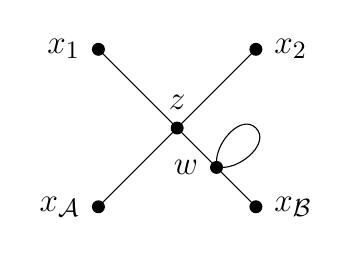
\begin{tikzpicture}
        \begin{feynman}
            \node[dot, label=above:\(z\)](z) at (0, 0);
            \node[dot, label=left:\(x_\mathcal{A}\)](i1) at (-1, -1);
            \node[dot, label=right:\(x_\mathcal{B}\)](i2) at (1, -1);
            \node[dot, label=left:\(x_1\)](f1) at (-1, 1);
            \node[dot, label=right:\(x_2\)](f2) at (1, 1);
            \node[dot, label=left:\(w\)](w) at (0.5, -0.5);
            \vertex(w0) at (1, 0);
            \diagram*{
                (i1) -- (z),
                (i2) -- (w),
                (w) -- (z),
                (z) -- (f1),
                (z) -- (f2),
                (w) --[out=0, in=-45] (w0),
                (w0) --[out=135, in=90] (w),
            };
        \end{feynman}
    \end{tikzpicture} \\
    =& \recip{2}(-i\lambda)^2
    \int\ud^4wD_F(x_\mathcal{B}-w)D_F(w-z)D_F(w-w) \\
    & \int\ud^4zD_F(x_1-z)D_F(x_2-z)D_F(x_\mathcal{A}-z)D_F(w-z) \\
    =& \recip{2}(-i\lambda)^2
    \int\ud^4w
    \int\frac{\ud^4p_\mathcal{B}}{(2\pi)^4}\frac{i}{p_\mathcal{B}^2-m^2+i\epsilon}e^{-ip_\mathcal{B}\cdot(x_\mathcal{B}-w)} \\
    & \int\frac{\ud^4p^\prime}{(2\pi)^4}\frac{i}{{p^\prime}^2-m^2+i\epsilon}e^{+ip^\prime\cdot(z-w)} \\
    & \int\frac{\ud^4k}{(2\pi)^4}\frac{i}{k^2-m^2+i\epsilon}e^{-ik\cdot(w-w)} \\
    & \cdot\int\ud^4z
    \int\frac{\ud^4p_\mathcal{A}}{(2\pi)^4}\frac{i}{p_\mathcal{A}^2-m^2+i\epsilon}e^{-ip_\mathcal{A}\cdot(x_\mathcal{A}-z)} \\
    & \int\frac{\ud^4p^\prime}{(2\pi)^4}\frac{i}{{p^\prime}^2-m^2+i\epsilon}e^{-ip^\prime\cdot(w-z)} \\
    & \int\frac{\ud^4p_1}{(2\pi)^4}\frac{i}{p_1^2-m^2+i\epsilon}e^{+ip_1\cdot(x_1-z)} \\
    & \int\frac{\ud^4p_2}{(2\pi)^4}\frac{i}{p_2^2-m^2+i\epsilon}e^{+ip_2\cdot(x_2-z)} \\
    =& \recip{2}(-i\lambda)^2
    \int\frac{\ud^4p_\mathcal{B}}{(2\pi)^4}\frac{i}{p_\mathcal{B}^2-m^2+i\epsilon} \\
    & \int\frac{\ud^4p^\prime}{(2\pi)^4}\frac{i}{{p^\prime}^2-m^2+i\epsilon} \int\frac{\ud^4k}{(2\pi)^4}\frac{i}{k^2-m^2+i\epsilon} \\
    & \cdot \int\frac{\ud^4p_\mathcal{A}}{(2\pi)^4}\frac{i}{p_\mathcal{A}^2-m^2+i\epsilon} \int\frac{\ud^4p^\prime}{(2\pi)^4}\frac{i}{{p^\prime}^2-m^2+i\epsilon} \\
    & \int\frac{\ud^4p_1}{(2\pi)^4}\frac{i}{p_1^2-m^2+i\epsilon} \int\frac{\ud^4p_2}{(2\pi)^4}\frac{i}{p_2^2-m^2+i\epsilon} \\
    & \cdot (2\pi)^4\delta^{(4)}(p_\mathcal{B}-p^\prime)(2\pi)^4\delta^{(4)}(p_\mathcal{A}+p^\prime-p_1-p_2)
}

Using LSZ reduction formula at Schwartz 6.19 and Peskin 7.42:

\eqnum{
    \brakaket{p_3\dots p_n}{S}{p_1p_2} =& \left[
        i\int\ud^4x_1e^{-ip_1x_1}(\DAlambert_1+m^2)
    \right]\dots\left[
        i\int\ud^4x_ne^{+ip_nx_n}(\DAlambert_n+m^2)
    \right] \\
    & \brakaket{\Omega}{T\{\phi(x_1)\phi(x_2)\phi(x_3)\dots\phi(x_n)\}}{\Omega},
}

where $\DAlambert = (\dpartial{}{x^\mu})^2 = \partial_t^2-\vec{\partial}_x^2$.

The above diagram's contributing to

\eqnum{
    \brakaket{\Omega}{T\{\phi(x_\mathcal{A})\phi(x_\mathcal{B})\phi(x_1)\phi(x_2)\}}{\Omega}
}

is:

\eqnum{
    & 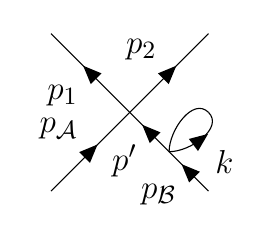
\begin{tikzpicture}
        \begin{feynman}
            \vertex (p) at (0, 0);
            \vertex(i1) at (-1, -1);
            \vertex(i2) at (1, -1);
            \vertex(f1) at (-1, 1);
            \vertex(f2) at (1, 1);
            \vertex(k) at (0.5, -0.5);
            \vertex(k0) at (1, 0);
            \diagram*{
                (i1) --[fermion, edge label=\(p_\mathcal{A}\)] (p),
                (i2) --[fermion, edge label=\(p_\mathcal{B}\)] (k),
                (k) --[fermion, edge label=\(p^\prime\)] (p),
                (p) --[fermion, edge label=\(p_1\)] (f1),
                (p) --[fermion, edge label=\(p_2\)] (f2),
                (k) --[fermion, out=0, in=-45, edge label'=\(k\)] (k0),
                (k0) --[out=135, in=90] (k),
            };
        \end{feynman}
    \end{tikzpicture} \\
    =& \half{1}
    \int\frac{\ud^4p^\prime}{(2\pi)^4}\frac{i}{{p^\prime}^2-m^2}
    \int\frac{\ud^4k}{(2\pi)^4}\frac{i}{k^2-m^2} \\
    & \times(2\pi)^4\delta^{(4)}(p_\mathcal{B}-p^\prime)(2\pi)^4\delta^{(4)}(p_\mathcal{A}+p^\prime-p_1-p_2)
}

where the external particles' Feynman propagators are cancelled. Because the $\partial_t^2$ yields 0 and $i$ in LSZ reduction formula are factored out by $\DAlambert^2+m^2$.

\subsubsection{4.107}

Revisit the equation 4.107:

Given equation 3.99 and 3.100, Dirac field operators in \textit{interaction picture} are:

\eqnum{
    \psi(x) =& \int\frac{\ud^3p}{(2\pi)^3}\recip{\sqrt{2E_\bf{p}}}\sum_s\left(
        a_\bf{p}^su^s(p)e^{-ip\cdot x} + b_\bf{p}^{s\dagger}v^s(p)e^{ip\cdot x}
    \right) \\
    \bar{\psi}(x) =& \int\frac{\ud^3p}{(2\pi)^3}\recip{\sqrt{2E_\bf{p}}}\sum_s\left(
        b_\bf{p}^s\bar{v}^s(p)e^{-ip\cdot x} + a_\bf{p}^{s\dagger}\bar{u}^s(p)e^{ip\cdot x}
    \right).
}

Decompose the Dirac field operators into positive- and negative- frequency parts:

\eqnum{
    \psi(x) =& \psi^+(x) + \psi^-(x) \\
    \bar{\psi}(x) =& \bar{\psi}^+(x) + \bar{\psi}^-(x),
}

where

\eqnum{
    \psi^+(x) =& \int\frac{\ud^3p}{(2\pi)^3}\recip{\sqrt{2E_\bf{p}}}\sum_s a_\bf{p}^su^s(p)e^{-ip\cdot x} \\
    \psi^-(x) =& \int\frac{\ud^3p}{(2\pi)^3}\recip{\sqrt{2E_\bf{p}}}\sum_s b_\bf{p}^{s\dagger}v^s(p)e^{ip\cdot x} \\
    \bar{\psi}^+(x) =& \int\frac{\ud^3p}{(2\pi)^3}\recip{\sqrt{2E_\bf{p}}}\sum_s b_\bf{p}^s\bar{v}^s(p)e^{-ip\cdot x} \\
    \bar{\psi}^-(x) =& \int\frac{\ud^3p}{(2\pi)^3}\recip{\sqrt{2E_\bf{p}}}\sum_s a_\bf{p}^{s\dagger}\bar{u}^s(p)e^{ip\cdot x}.
}

Similar to 4.33, if $x^0>y^0$,

\eqnum{
    & T\left[\psi(x)\bar{\psi}(y)\right] \\
    =& \psi^+(x)\bar{\psi}^-(y) + \bar{\psi}^-(y)\psi^+(x) + \psi^-(x)\bar{\psi}^+(y) + \psi^-(x)\bar{\psi}^+(y) + \left[\psi^+(x), \bar{\psi}^-(y)\right].
}

So, based on 3.114 and 3.121,

\eqnum{
    \brakaket{0}{T\left[\psi(x)\bar{\psi}(y)\right]}{0} =& \brakaket{0}{N\left[\psi(x)\bar{\psi}(y)\right]}{0} + \brakaket{0}{\left[\psi^+(x), \bar{\psi}^-(y)\right]}{0} \\
    \brakaket{0}{\left[\psi^+(x), \bar{\psi}^-(y)\right]}{0}
    =& \int\frac{\ud^3p}{(2\pi)^3}\recip{2E_\bf{p}}\sum_s u^s\bar{u}^s e^{-ip\cdot (x-y)} + 0 \\
    =& \brakaket{0}{\psi(x)\bar{\psi}(y)}{0} = \brakaket{0}{\{\psi^+(x), \bar{\psi}^-(y)\}}{0},
}

because in $\brakaket{0}{\bar{\psi}^-(y)\psi^+(x)}{0}$ all the $a_\bf{p}$ are at the right of all the $a^\dagger_\bf{p}$.

Similarly, when $x^0<y^0$, based on 3.115 and 3.121,

\eqnum{
    \brakaket{0}{T\left[\bar{\psi}(y)\psi(x)\right]}{0} =& \brakaket{0}{N\left[\bar{\psi}(y)\psi(x)\right]}{0} + \brakaket{0}{\left[\bar{\psi}^+(y), \psi^-(x)\right]}{0} \\
    \brakaket{0}{\left[\bar{\psi}^+(y), \psi^-(x)\right]}{0} =& -\brakaket{0}{\bar{\psi}(y)\psi(x)}{0} \\
    =& -\brakaket{0}{\{\bar{\psi}^+(y), \psi^-(x)\}}{0}.
}

So that

\eqnum{
    S_F(x-y) = \begin{cases}
        \brakaket{0}{\{\psi^+(x), \bar{\psi}^-(y)\}}{0}\ \mathrm{for}\ x^0>y^0 \\
        -\brakaket{0}{\{\bar{\psi}^+(y), \psi^-(x)\}}{0}\ \mathrm{for}\ x^0<y^0
    \end{cases}
}

and 

\eqnum{
    T\left[\psi(x)\bar{\psi}(y)\right] =& N\left[\psi(x)\bar{\psi}(y)\right] + \wick{\c \psi(x)\bar{\c \psi}(y)} \\
    =& S_F(x-y).
}


% \input{template}

\end{document}
